\documentclass[]{standalone}

\usepackage{../lenses}
\usepackage{ifthen}


\newcommand{\lenseGeneric}[7]{ % symm,a1,a2,a3,size,rot,color
 \pgfmathsetmacro\symm{360/#1}
 \pgfmathsetmacro\aa{180-(#2*\symm)}
 \pgfmathsetmacro\ab{180-(#3*\symm)}
 \pgfmathsetmacro\ac{180-(#4*\symm)}
 \pgfmathsetmacro\ca{#5*cos(\ac)}
 \pgfmathsetmacro\sa{#5*sin(\ac)}
 \pgfmathsetmacro\cb{#5*cos(\ac+\ab))}
 \pgfmathsetmacro\sb{#5*sin(\ac+\ab)}
 \pgfmathsetmacro\cc{#5*cos(\ac+\ab+\aa)}
 \pgfmathsetmacro\sc{#5*sin(\ac+\ab+\aa)}
 \pgfmathsetmacro\cd{#5*cos(\ac+\ab+\aa+\ac)}
 \pgfmathsetmacro\sd{#5*sin(\ac+\ab+\aa+\ac)}
 \begin{scope}[rotate=#6*\symm/2]
  \definecolor{main}{HTML}{#7}
  \fill[main] (0,0)
  -- ++(#5,0)
  -- ++(\ca,\sa)
  -- ++(\cb,\sb)
  -- ++(\cc,\sc)
  -- ++(\cd,\sd)
  -- cycle;
  \draw[] (0,0)
  -- ++(#5,0)
  -- ++(\ca,\sa)
  -- ++(\cb,\sb)
  -- ++(\cc,\sc)
  -- ++(\cd,\sd)
  -- cycle;
 \end{scope}
}

\newcommand{\lenseDD}[4]{ %size,rot,color,letter
 \lenseGeneric{7}{1}{3}{3}{#1}{#2}{#3}
 \ifthenelse{#4=0}{}{
  \begin{scope}[rotate=#2*360/14 + 180/7]
   \draw(#1*1.5,0) node{\textbf{\em D}};
  \end{scope}
 }
}

\newcommand{\lenseEE}[4]{ %size,rot,color,letter
 \lenseGeneric{7}{1}{2}{4}{#1}{#2}{#3}
 \ifthenelse{#4=0}{}{
  \begin{scope}[rotate=#2*360/14 + 180/14]
   \draw(#1*1.1,0) node{\textbf{\em E}};
  \end{scope}
 }
}


\begin{document}
 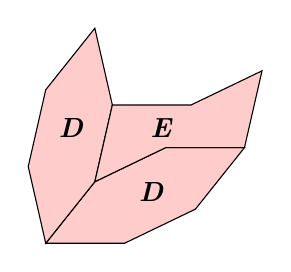
\begin{tikzpicture}
  \begin{scope}[scale=1]
  
   \lenseDD{1}{0}{FFCCCC}{1} %size,rot,color,letter
   \lenseDD{1}{2}{FFCCCC}{1}

   \begin{scope}[rotate=360/7,shift={(1,0)}] \lenseEE{1}{-1}{FFCCCC}{1} \end{scope}
    
  
  
  
%   \definecolor{leaf}{HTML}{FFCCCC} % pink
%   \definecolor{moon}{HTML}{CCFFCC} % green
%   \definecolor{crown}{HTML}{CCCCFF} % blue
%   \pgfmathsetmacro\side{1}
%   \pgfmathsetmacro\a{180/7}
%   \pgfmathsetmacro\ca{\side*cos(\a)}
%   \pgfmathsetmacro\sa{\side*sin(\a)}
%   \pgfmathsetmacro\cb{\side*cos(2*\a)}
%   \pgfmathsetmacro\sb{\side*sin(2*\a)}
%   \pgfmathsetmacro\cc{\side*cos(3*\a)}
%   \pgfmathsetmacro\sc{\side*sin(3*\a)}
%   \begin{scope}[shift={(0,-1)}]
%    \begin{scope}[]
%     \draw[crown] (0,0) % C+C
%      -- ++(-\cc,\sc)
%      -- ++(\cc,\sc)
%      -- ++(\side,0)
%      -- ++(\cc,-\sc)
%      -- ++(\cb,-\sb)
%      -- ++(\ca,\sa)
%      -- ++(-\cc,\sc)
%      -- ++(\ca,-\sa)
%      -- ++(-\ca,-\sa)
%      -- ++(\cc,-\sc)
%      -- ++(-\ca,\sa)
%      -- cycle;
%      \fill[leaf] (\side,0)
%       -- ++(\cc,\sc)
%       -- ++(-\cc,\sc)
%       -- ++(\ca,\sa)
%       -- ++(-\cc,-\sc)
%       -- ++(\cc,-\sc)
%       -- cycle;
%
%     \lenseD{000000}{\side}{1} % DEF-leaf
%     \begin{scope}[rotate=\a]
%      \lenseD{000000}{\side}{1} 
%      \begin{scope}[shift={(\side,0)}]
%       \begin{scope}[rotate=-0.5*\a] 
%        \lenseE{000000}{\side}{1}
%        \begin{scope}[rotate=\a,shift={(\side,0)},rotate=-1.5*\a]
%         \lenseF{000000}{\side}{1}
%         %\draw(0,0) node{$o$};
%        \end{scope}
%       \end{scope}
%      \end{scope}    
%     \end{scope}    
%
%     %\begin{scope}[shift={(\side,0)},rotate=36] \lenseB{000000}{\side}{1} \end{scope}    
%     %\begin{scope}[shift={(\side,0)},rotate=-36] \lenseC{000000}{\side}{1} \end{scope}    
%    \end{scope}
%    \draw (1,-1) node{$(i)$};
%   \end{scope}
%   
%   \begin{scope}[shift={(4,0)}] % regular decagon
%    \begin{scope}[]
%    \fill[leaf] (0,0)
%     -- ++(\cb,\sb)
%     -- ++(\ca,\sa)
%     -- ++(\side,0)
%     -- ++(-\cb,-\sb)
%     -- ++(-\ca,-\sa)
%     -- cycle;
%     \lenseB{000000}{\side}{1}
%     
%     \fill[moon] (\side,0)
%     -- ++(\ca,\sa)
%     -- ++(\cb,\sb)
%     -- ++(\ca,-\sa)
%     -- ++(-\cc,-\sc)
%     -- ++(\cc,-\sc)
%     -- ++(-\ca,-\sa)
%     -- ++(-\side,0)
%     -- ++(-\ca,\sa)
%     -- ++(-\cb,\sb)
%     -- cycle;
%     
%     \begin{scope}[rotate=-72] \lenseB{000000}{\side}{1} \end{scope}   
%     \begin{scope}[shift={(\side,0)},rotate=-36] \lenseC{000000}{\side}{1} \end{scope}   
%     \begin{scope}[shift={(\side,0)},rotate=-36]
%      \begin{scope}[shift={(\side,0)},rotate=-36]
%       \begin{scope}[shift={(\side,0)},rotate=-36+144]
%        \lenseB{000000}{\side}{1}
%       \end{scope}
%      \end{scope}
%     \end{scope}   
%    \end{scope}   
%    \draw (1.5,-2) node{$(ii)$};
%   \end{scope}
%  
  \end{scope}
 \end{tikzpicture}
\end{document}